%% This is an example first chapter.  You should put chapter/appendix that you
%% write into a separate file, and add a line \include{yourfilename} to
%% main.tex, where `yourfilename.tex' is the name of the chapter/appendix file.
%% You can process specific files by typing their names in at the 
%% \files=
%% prompt when you run the file main.tex through LaTeX.
\justify
\chapter{3. Extended Examples}

\section{Traditional methods for community engagement}

\subsection{Attempts from Architects and Planners}

The objective of an Architect or a Planner is to take into account various
aspects of a problem and consolidate into an actionable plan.
The knowledge give hints how we can construct an integrated method or
participatory urban design.

\textbf{Lawrance Halprin & Charles Moore} \\
Lawrance Halprin & Charles Moore have concentrated on trying different methodologies of collaborative creative processes.
For designing large scale projects, they used a large canvas to draw the
plan or perspective within the community meeting iterating through the
different design possibilities. This method illustrates the designer's role
of integration.

Landscape Architect Lawrence Halprin also proposed the RVSP Cycle; a method
of a collaborative creative process and practiced throughout his career. It
is a circular diagram inspired on the compass of psyche from Jung.

\begin{table}
  \centering
  \begin{tabular}{c|c|c}
    R & resource & data collection phase to know what is available \\
    S & score & the instruction set for the intervention \\
    V & value-action & a collective process of debating and discussion \\
    P & performance & the execution of the plan \\
  \end{tabular}
  \caption{elements of the RSVP cycles}
  \label{tab:rvsp}
\end{table}:w

The creator argues that this cycle is agnostic to where it starts or the
order of execution of each element. Halprin also emphasizes that this is an
endless process which changes its coordinate relatively to the steps taken
chronologically. This relativeness comes from the influence by his wife
Anna Halprin which was a choreographer. This behavior resembles and can
consider as a similar strategy as a search algorithm trying to look for a
(sub) optimum while the fitness landscape changes in the same time. Which
illustrates the “wickedness”.

\begin{marginfigure}
  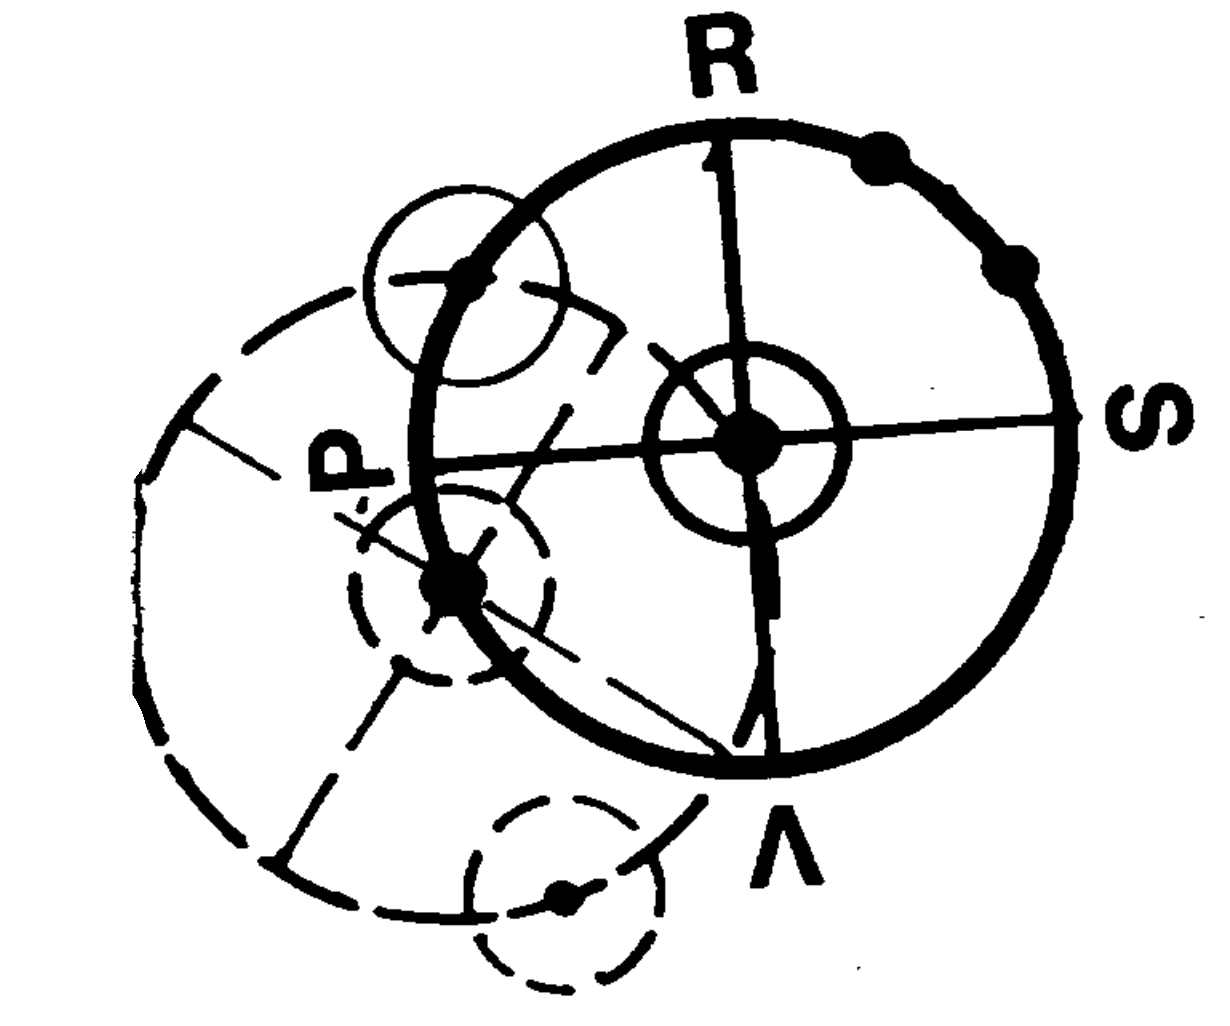
\includegraphics[width=\textwidth]{chapters/3/fig/rvsp_relative.png}               
  \caption{the RVSP cycle changes its position dynamically, relative to
  the previous state \cite{halprin1969rsvp}}
  \label{fig:spin_margin}
\end{marginfigure}

\textbf{Arata Isozaki}
Architect Isozaki Arata held an exhibition in 1997 using the internet and
email for planning, which is one of the earliest examples for collectively
designing an urban scale project by both citizen and professional
collaboration using new media.
A fictitious island was the site for this design iteration with three
methods for this participatory approach; each art piece named ``the
internet'', ``visitors'' and ``signatures.'' 
``The internet'' was the open platform that will let opinions from the public
modify the virtual plan. While the number of people connected to the web in
Japan was only around 10\% of the total population, at that year, the
exhibition was open for gathering opinions via email and provided 3D models
to modify or overwrite the existing design.\footnote{Information Technology White Paper
\url{http://www.soumu.go.jp/johotsusintokei/whitepaper/ja/h27/html/nc372110.html}}
“Signatures” had 50 architects assigned a site separately planned one of
their previous architectural pieces without any consideration. The initial
layout plan triggers problems that will need negotiation between adjacent
architects to `fit' their design properly.
``Visitors'' focused on the chronological aspect of collaborative design.
It had a chief architect that will supervise one district for a total of
two weeks, passing it to the next architect after their turn. This workflow
has similarities in today's software development where people
collaboratively develop software by forking code made by peers. The
architect was encouraged to collect data from the internet.
This exhibition was not only novel because of using the internet and email
but was an experiment on how we collaborate and interact using these new
techniques.

\subsection{Known Traditional Methods}
Appendix \ref{app:traditional} shows different methods of traditional community engagement.

\subsection{Browser based applications}

\textbf{Nigechizu -Short cut Evacuation Planning fro Tsunami-}

\begin{figure}[htb]
  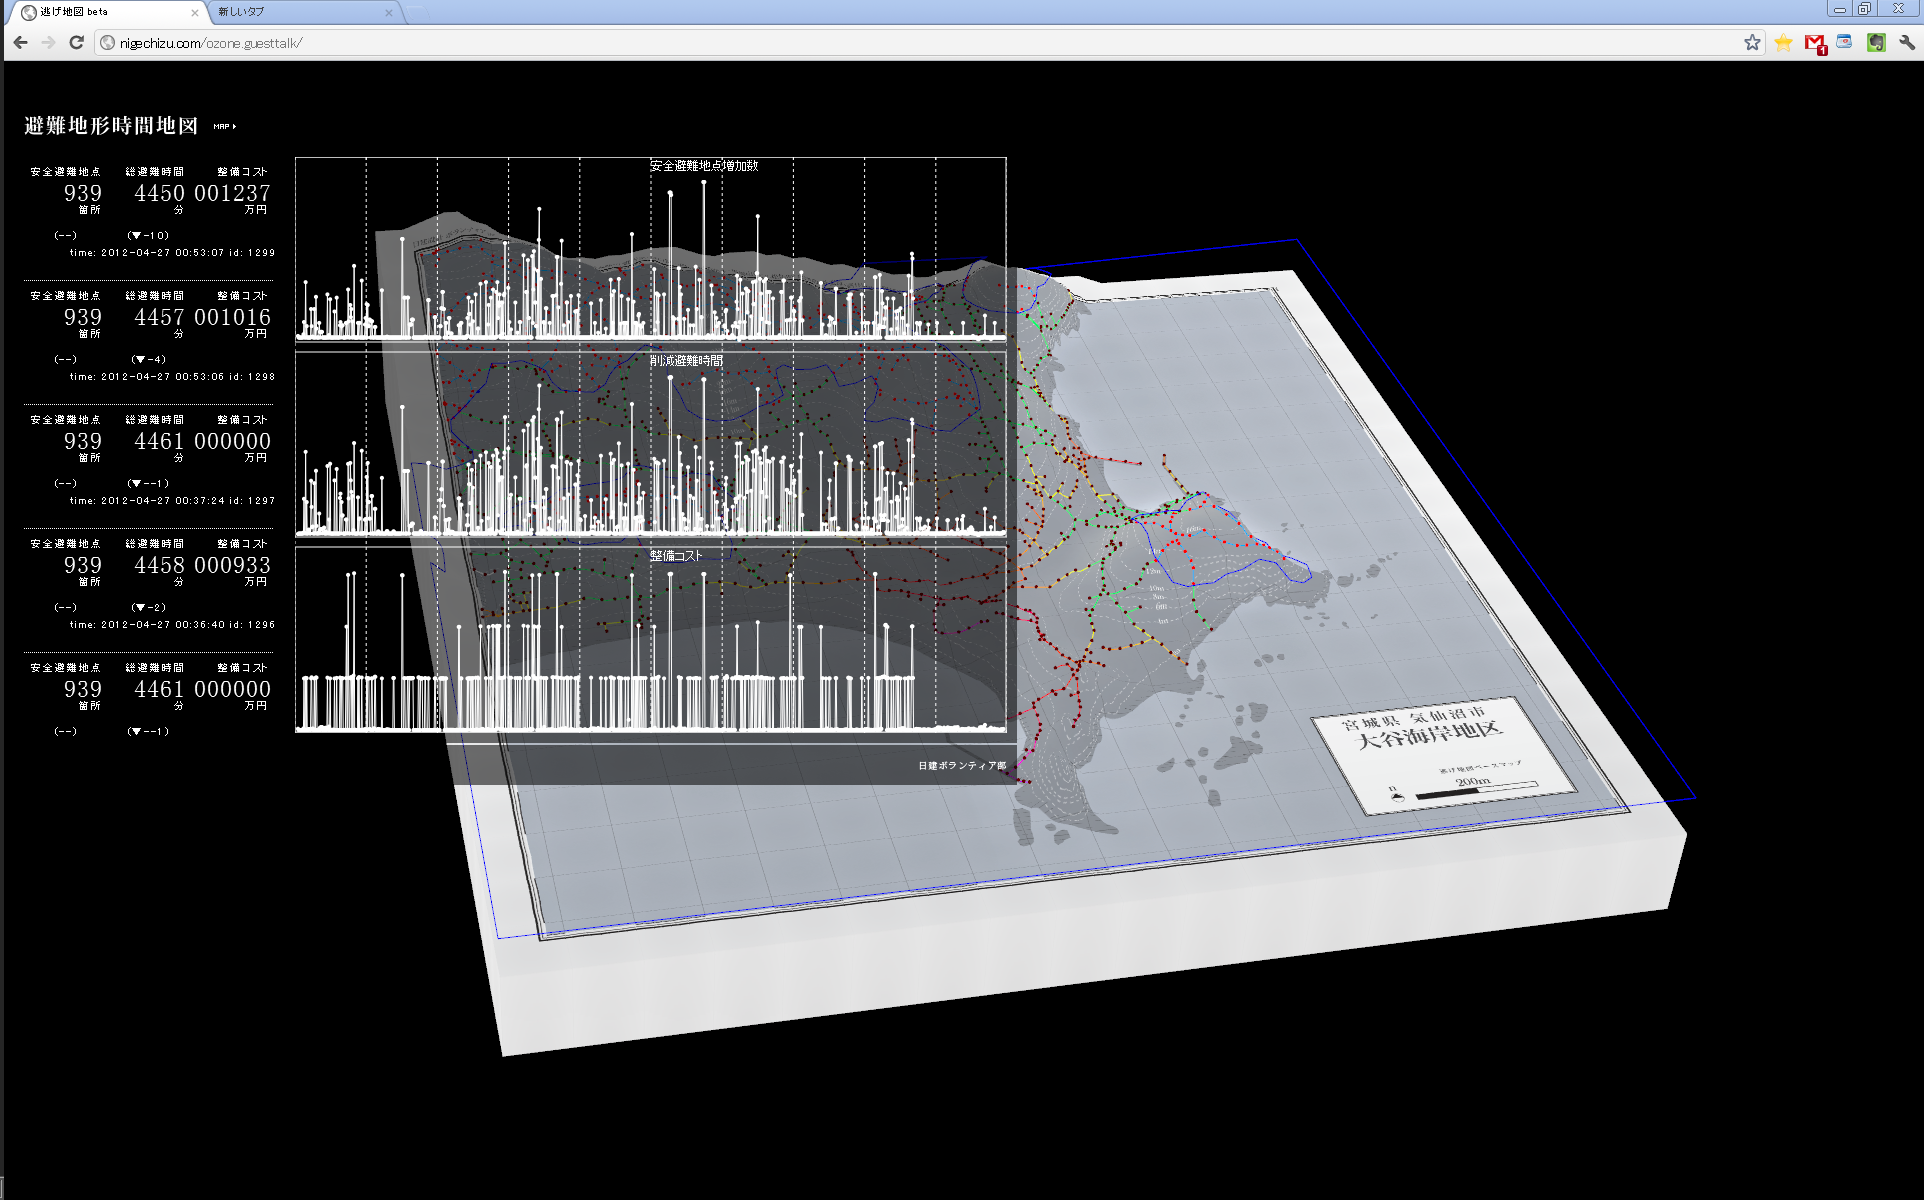
\includegraphics[width=\textwidth]{chapters/3/fig/nigechizu002.png}               
  \caption[nigechizu]{\textfb{Web based short cut planning tool} created
  for workshops to learn the risks of tsunami and how to evacuate.}
  \label{fig:nigechizu}
\end{figure}

Reflecting the tsunami damage from 2011 Tohoku Earthquake and tsunami, I have created this tool as a community engagement tool.

This web browser based tool starts by visualizing the risk of a tsunami
coloring the paths depending on the duration for evacuation.
\footnote{this was calculated by a normal walking speed of a elderly, taking the shortest
path to the closest high enough altitude.}
After the first strike of the tsunami, people constantly wanted to know
which direction to escape because it was sometimes not obvious given the
compound terrain.
The second feature was to let the community choose were to create
shortcuts.
Since shortcuts paths reduce the time for an evacuation, it increases the area's safety
level as a whole. The distinctive feature of this app is enabling people
choosing two points to connect, unlike voting for a particular
configuration. The trials were recorded in the server to be super imposed
to get the most popular positions that needed to be connected.

\begin{marginfigure}[{0cm}]
  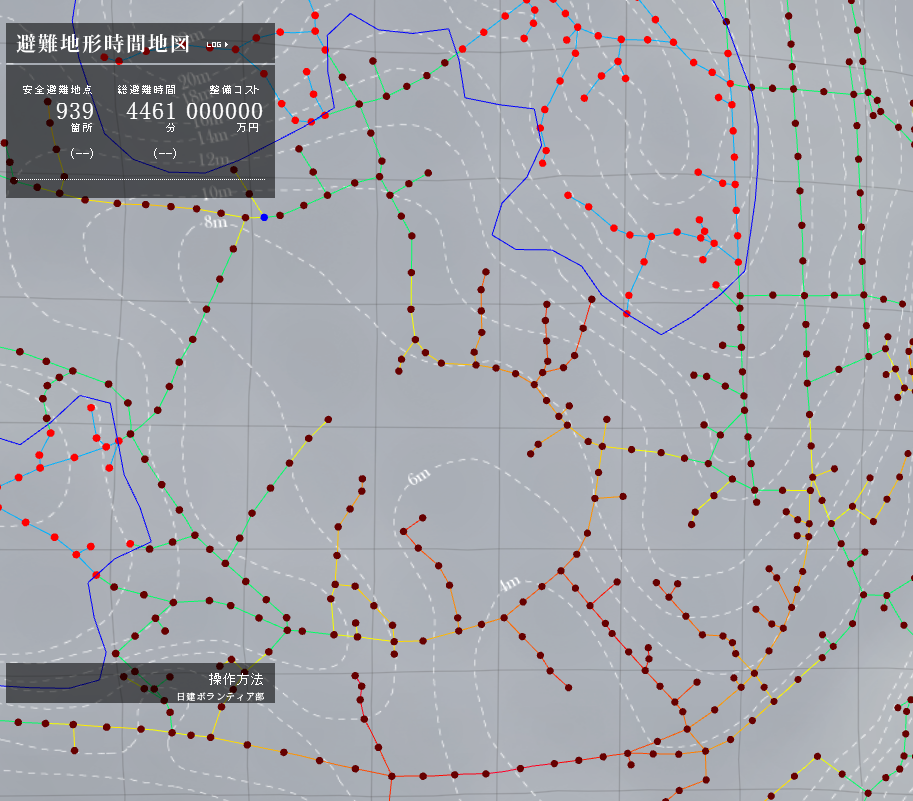
\includegraphics[width=\textwidth]{chapters/3/fig/nigechizu001.png}               
  \caption[zoom in nigechizu interface]{Users will connect two points to create a shortcut to decrease the overall evacuation time.}
  \label{fig:nigechizu}
\end{marginfigure}

\begin{marginfigure}[{0cm}]
  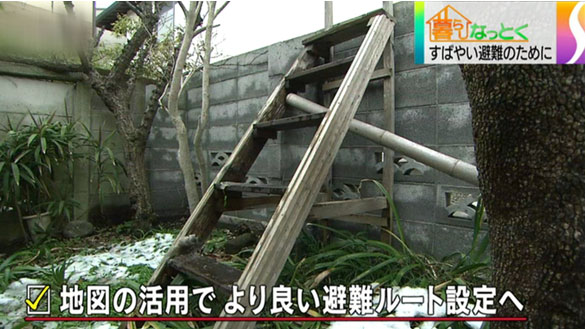
\includegraphics[width=\textwidth]{chapters/3/fig/nhk_kamakura.jpg}               
  \caption[collective collaboration]{After one of the workshops neighbors
  negotiated with each other and installed a wooden staircase to be used as
a general asset for emergency evacuation. \url{https://www3.nhk.or.jp}}
  \label{fig:nigechizu}
\end{marginfigure}


\textbf{LMN Architects -distributed version controlling in 3d
models-}

Lmn architecture is a 3d modeling app in a web browser, and that every
model is connected forming a network.
The connection of two models is the inheritance, where the participants
choose a pre existing model as a reference and start modeling on top.
The unit data that each user sends in one interaction is a 3d model, which
is large (compared to voting) and often thought as unstructured data. The
app saves the 3d model into a data structure that could apply a diff
algorithm to make the 3d model comparable and calculate the similarity
between two models visualizing the strength of the connection.

\begin{figure}[htb]
  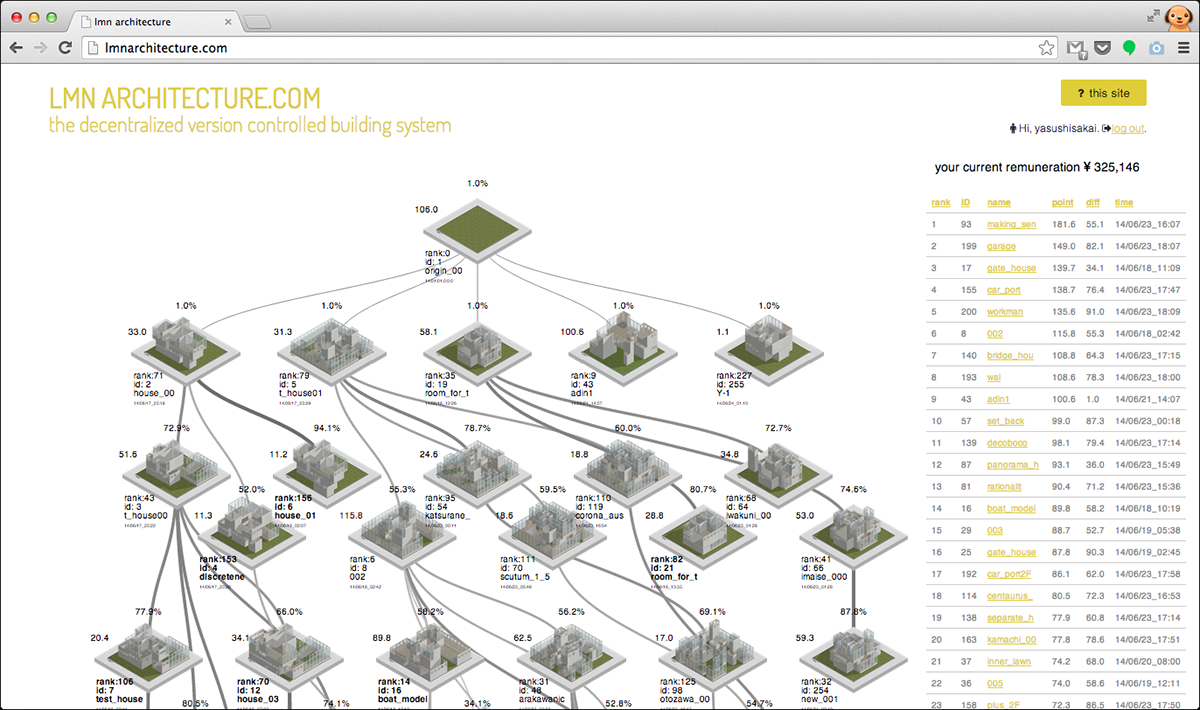
\includegraphics[width=\textwidth]{chapters/3/fig/lmn_004.png}               
  \caption[LMN:web based distributed modelling]{Web based distributed modeling}
  \label{fig:lnm}
\end{figure}

\begin{marginfigure}[{0cm}]
  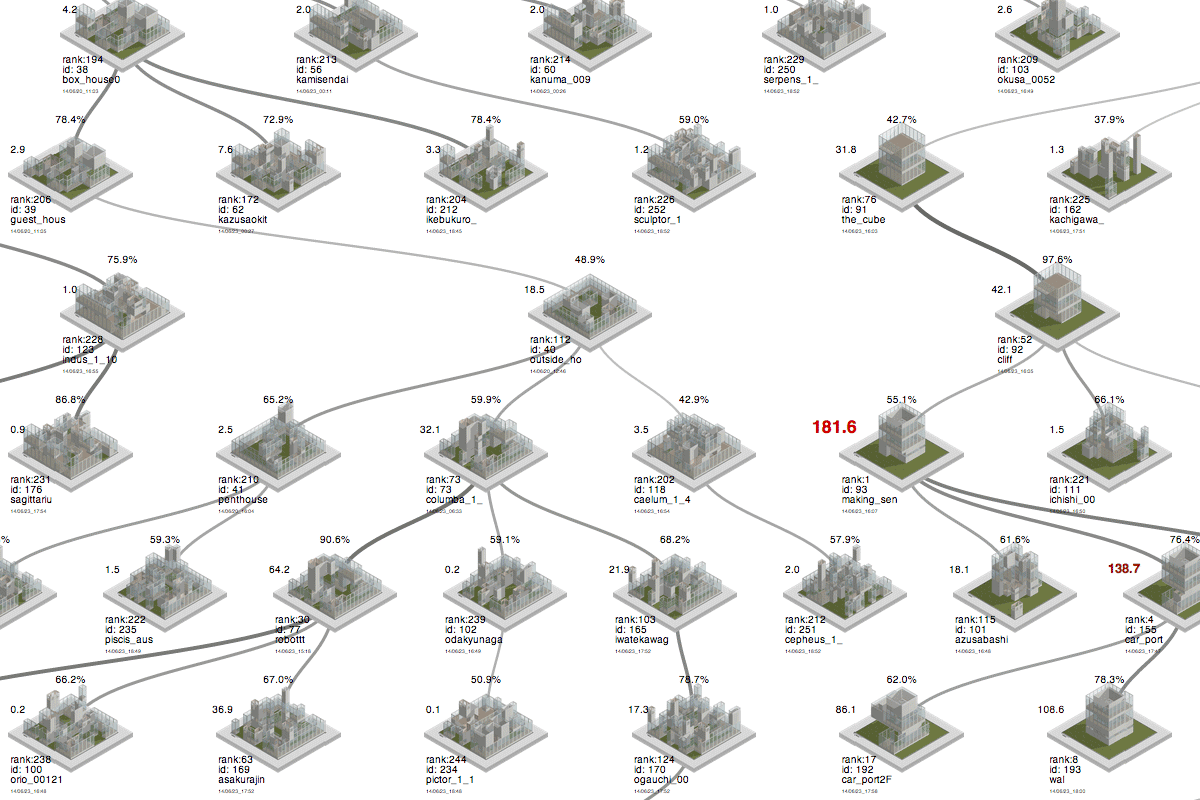
\includegraphics[width=\textwidth]{chapters/3/fig/lmn_000.png}               
  \caption[LMN:net work of models]{Each model starts with a preexisting
  model and revises it. Thus every model is connected having the similarity
calculated by the diff algorithm}
  \label{fig:lnm_zoom}
\end{marginfigure}

\begin{marginfigure}[{0cm}]
  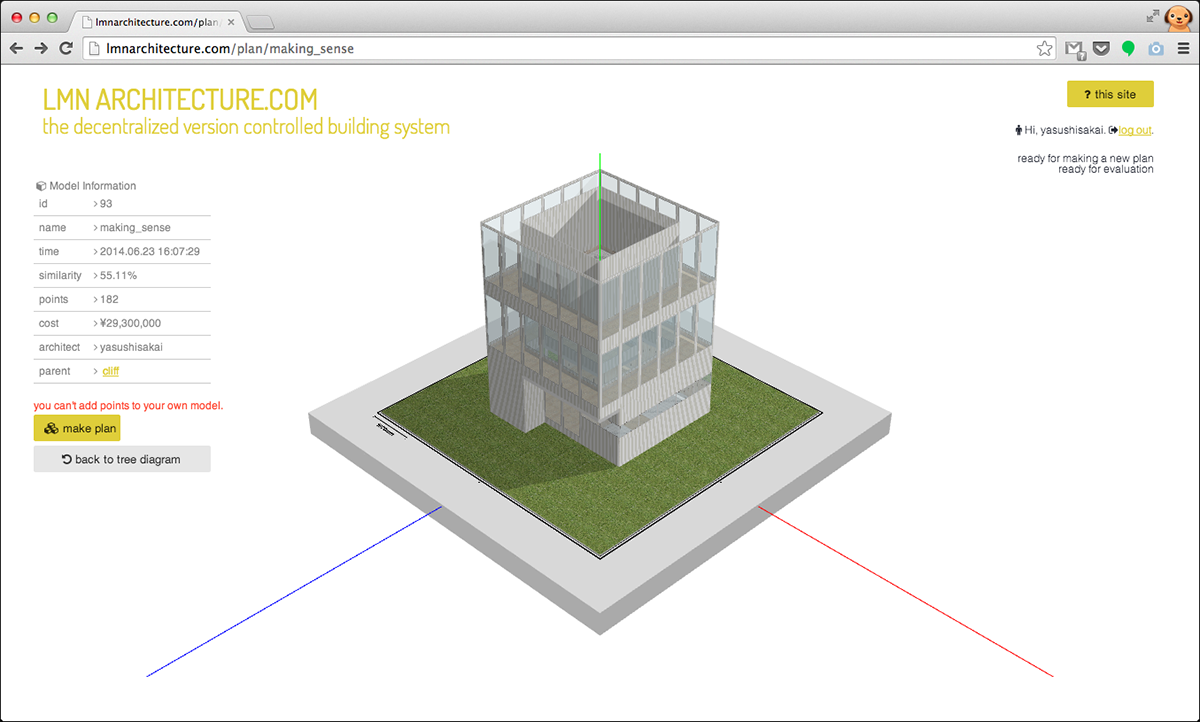
\includegraphics[width=\textwidth]{chapters/3/fig/lmn_006.png}               
  \caption[LMN: modeling inside the browser]{Every model is created using the web browser.}
  \label{fig:lnm_create}
\end{marginfigure}

\textbf{PlacePulse}\\
Place Pulse\footnote{\url{http://pulse.media.mit.edu/}}\cite{salesses2013collaborative} developed
by the Collective Learning Group in MIT Media Lab, is a collective effort
to map our perception about the city by selecting one image out of two.
\footnote{or both, meaning equal}
The amount of information sent per interaction is smallest in this section,
yet have collected more than 1.4 million clicks/footnote{as of August 2017}

\subsection{Mobile Applications}

% TODO: images
\textbf{BOS:311 app}\\

BOS 311 is a mobile app that lets you report city maintenance issues. The
number 311 is traditionally a phone number that citizens can call when
their maintenance was required. Reporters can submit text and pictures,
which is unconstrained. The reports focus on maintenance issues, less about
the planning and changing the city.

\textbf{Waze}\\
Waze is a driving navigation app, which uses the status of other drivers
using the same app. Each driver can passively send the location and speed
of the car, or actively contribute to marking the road if there is
something worth to notice other drives. Each data is structured. 
This distributed traffic monitoring is an example of collective analysis,
creating trust and mutual benefit between complete strangers who do not
share any identity except being drivers.
Since the objective of this app is to form this collective intelligence,
there is no connection to any planning procedure.

\textbf{Action Path}\\
Action Path\footnote{\url{http://actionpath.org/}} \cite{graeff2014crowdsourcing} developed at
the Center for Civic Media, is a mobile app that shows notifications when a
user enters a predefined geolocation and asking questions on urban issues
tied to that geolocation. The app provides agency to the citizens and
creates data to represent the collective opinion. A small amount of data
sent for each interaction geolocation and the answer.

\subsection{Tangible Interfaces: CityScope}

City Scope is a platform for people to gather and build consensus with a
device having data projections, a tangible interface, and real-time
simulation. Multiple projects have advanced using this platform
collaboration with different cities and universities. Each project has a
different focus hence the contents/footnote{what to visualize/project, type
of simulation, who to engage, objective} has varied.

\textbf{Finding Places}

Finding Places is one of them targeting the issue of allocating
immigrants\footnote{Germany received more than 1.2million refugees in 2015.} that
entered Hamburg, Germany. Using City Scope, a total of 34 workshops was
conducted to discuss the best place to open room for those seeking asylum.
Each session took 2 hours with on average 11 people participating.

This tool covers the analytical phase and synthetic phase and enables
people to have real-time feedback running simulations showing potential
implications of the population increase. It is a structured tool since
users manipulate color coded lego bricks to run each simulation. On the
other hand, the discussion held over the table is rich and vocal.

\begin{figure}[htb]
  
\includegraphics[width=\textwidth]{chapters/3/fig/cityscope.png}               
  \caption[diagram: cityscope]{Changing Places City Scope Platform}
  \label{fig:diagram_cityscope}
\end{figure}

% TODO: table for categorization
